\chapter{Data Recording}
To record data to train the classifier for a gesture, follow these steps:\\

\begin{figure}[H]
    \centering
    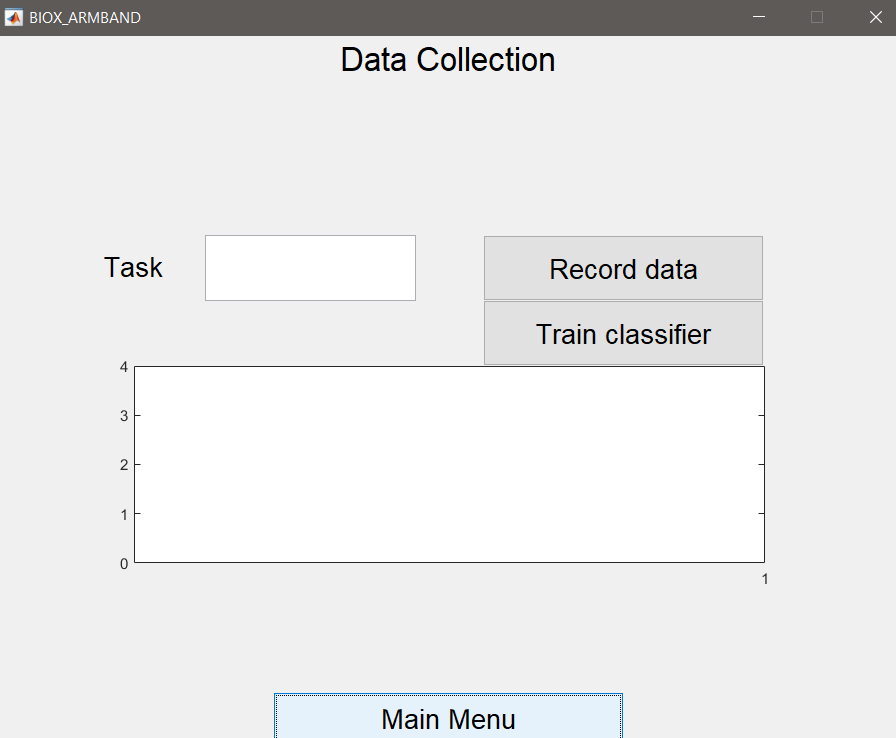
\includegraphics[width=0.6\linewidth]{figures/AppPics/4_DataRecording1.PNG}
    \caption{Data Recording menu.}
    \label{fig:my_label}
\end{figure}

\begin{enumerate}[label=\textbf{Step \arabic*}:]
    \item \label{datrecloopstart} Specify a name for the gesture.
    \item Click \textbf{"Record Data"}, to begin recording training data.
    \item Perform the chosen gesture and hold it static for a few seconds.
    \item Now, click \textbf{"Stop Recording"} again to stop the recording. 
    \item \label{datrecloopend} You are now promted to chose an interval from the recording to use as training input. Do this by clicking with the mouse at the desired start and stop time, along the x-axis of the plot.
    \item Add more gestures by repeating \ref{datrecloopstart} to \ref{datrecloopend}
    \item To train the classifier, click \textbf{"Train Classifier"}. If no data is recorded, this button will be inactive.
    \item Click \textbf{"Main Menu"} to return to the main menu.
    
    
\end{enumerate}